% Options for packages loaded elsewhere
\PassOptionsToPackage{unicode}{hyperref}
\PassOptionsToPackage{hyphens}{url}
\PassOptionsToPackage{dvipsnames,svgnames,x11names}{xcolor}
%
\documentclass[
  12pt,
  letterpaper,
  DIV=11,
  numbers=noendperiod]{scrartcl}

\usepackage{amsmath,amssymb}
\usepackage{iftex}
\ifPDFTeX
  \usepackage[T1]{fontenc}
  \usepackage[utf8]{inputenc}
  \usepackage{textcomp} % provide euro and other symbols
\else % if luatex or xetex
  \usepackage{unicode-math}
  \defaultfontfeatures{Scale=MatchLowercase}
  \defaultfontfeatures[\rmfamily]{Ligatures=TeX,Scale=1}
\fi
\usepackage{lmodern}
\ifPDFTeX\else  
    % xetex/luatex font selection
  \setmainfont[]{Times New Roman}
  \setsansfont[]{Times New Roman}
\fi
% Use upquote if available, for straight quotes in verbatim environments
\IfFileExists{upquote.sty}{\usepackage{upquote}}{}
\IfFileExists{microtype.sty}{% use microtype if available
  \usepackage[]{microtype}
  \UseMicrotypeSet[protrusion]{basicmath} % disable protrusion for tt fonts
}{}
\makeatletter
\@ifundefined{KOMAClassName}{% if non-KOMA class
  \IfFileExists{parskip.sty}{%
    \usepackage{parskip}
  }{% else
    \setlength{\parindent}{0pt}
    \setlength{\parskip}{6pt plus 2pt minus 1pt}}
}{% if KOMA class
  \KOMAoptions{parskip=half}}
\makeatother
\usepackage{xcolor}
\setlength{\emergencystretch}{3em} % prevent overfull lines
\setcounter{secnumdepth}{-\maxdimen} % remove section numbering
% Make \paragraph and \subparagraph free-standing
\ifx\paragraph\undefined\else
  \let\oldparagraph\paragraph
  \renewcommand{\paragraph}[1]{\oldparagraph{#1}\mbox{}}
\fi
\ifx\subparagraph\undefined\else
  \let\oldsubparagraph\subparagraph
  \renewcommand{\subparagraph}[1]{\oldsubparagraph{#1}\mbox{}}
\fi

\usepackage{color}
\usepackage{fancyvrb}
\newcommand{\VerbBar}{|}
\newcommand{\VERB}{\Verb[commandchars=\\\{\}]}
\DefineVerbatimEnvironment{Highlighting}{Verbatim}{commandchars=\\\{\}}
% Add ',fontsize=\small' for more characters per line
\usepackage{framed}
\definecolor{shadecolor}{RGB}{241,243,245}
\newenvironment{Shaded}{\begin{snugshade}}{\end{snugshade}}
\newcommand{\AlertTok}[1]{\textcolor[rgb]{0.68,0.00,0.00}{#1}}
\newcommand{\AnnotationTok}[1]{\textcolor[rgb]{0.37,0.37,0.37}{#1}}
\newcommand{\AttributeTok}[1]{\textcolor[rgb]{0.40,0.45,0.13}{#1}}
\newcommand{\BaseNTok}[1]{\textcolor[rgb]{0.68,0.00,0.00}{#1}}
\newcommand{\BuiltInTok}[1]{\textcolor[rgb]{0.00,0.23,0.31}{#1}}
\newcommand{\CharTok}[1]{\textcolor[rgb]{0.13,0.47,0.30}{#1}}
\newcommand{\CommentTok}[1]{\textcolor[rgb]{0.37,0.37,0.37}{#1}}
\newcommand{\CommentVarTok}[1]{\textcolor[rgb]{0.37,0.37,0.37}{\textit{#1}}}
\newcommand{\ConstantTok}[1]{\textcolor[rgb]{0.56,0.35,0.01}{#1}}
\newcommand{\ControlFlowTok}[1]{\textcolor[rgb]{0.00,0.23,0.31}{#1}}
\newcommand{\DataTypeTok}[1]{\textcolor[rgb]{0.68,0.00,0.00}{#1}}
\newcommand{\DecValTok}[1]{\textcolor[rgb]{0.68,0.00,0.00}{#1}}
\newcommand{\DocumentationTok}[1]{\textcolor[rgb]{0.37,0.37,0.37}{\textit{#1}}}
\newcommand{\ErrorTok}[1]{\textcolor[rgb]{0.68,0.00,0.00}{#1}}
\newcommand{\ExtensionTok}[1]{\textcolor[rgb]{0.00,0.23,0.31}{#1}}
\newcommand{\FloatTok}[1]{\textcolor[rgb]{0.68,0.00,0.00}{#1}}
\newcommand{\FunctionTok}[1]{\textcolor[rgb]{0.28,0.35,0.67}{#1}}
\newcommand{\ImportTok}[1]{\textcolor[rgb]{0.00,0.46,0.62}{#1}}
\newcommand{\InformationTok}[1]{\textcolor[rgb]{0.37,0.37,0.37}{#1}}
\newcommand{\KeywordTok}[1]{\textcolor[rgb]{0.00,0.23,0.31}{#1}}
\newcommand{\NormalTok}[1]{\textcolor[rgb]{0.00,0.23,0.31}{#1}}
\newcommand{\OperatorTok}[1]{\textcolor[rgb]{0.37,0.37,0.37}{#1}}
\newcommand{\OtherTok}[1]{\textcolor[rgb]{0.00,0.23,0.31}{#1}}
\newcommand{\PreprocessorTok}[1]{\textcolor[rgb]{0.68,0.00,0.00}{#1}}
\newcommand{\RegionMarkerTok}[1]{\textcolor[rgb]{0.00,0.23,0.31}{#1}}
\newcommand{\SpecialCharTok}[1]{\textcolor[rgb]{0.37,0.37,0.37}{#1}}
\newcommand{\SpecialStringTok}[1]{\textcolor[rgb]{0.13,0.47,0.30}{#1}}
\newcommand{\StringTok}[1]{\textcolor[rgb]{0.13,0.47,0.30}{#1}}
\newcommand{\VariableTok}[1]{\textcolor[rgb]{0.07,0.07,0.07}{#1}}
\newcommand{\VerbatimStringTok}[1]{\textcolor[rgb]{0.13,0.47,0.30}{#1}}
\newcommand{\WarningTok}[1]{\textcolor[rgb]{0.37,0.37,0.37}{\textit{#1}}}

\providecommand{\tightlist}{%
  \setlength{\itemsep}{0pt}\setlength{\parskip}{0pt}}\usepackage{longtable,booktabs,array}
\usepackage{calc} % for calculating minipage widths
% Correct order of tables after \paragraph or \subparagraph
\usepackage{etoolbox}
\makeatletter
\patchcmd\longtable{\par}{\if@noskipsec\mbox{}\fi\par}{}{}
\makeatother
% Allow footnotes in longtable head/foot
\IfFileExists{footnotehyper.sty}{\usepackage{footnotehyper}}{\usepackage{footnote}}
\makesavenoteenv{longtable}
\usepackage{graphicx}
\makeatletter
\def\maxwidth{\ifdim\Gin@nat@width>\linewidth\linewidth\else\Gin@nat@width\fi}
\def\maxheight{\ifdim\Gin@nat@height>\textheight\textheight\else\Gin@nat@height\fi}
\makeatother
% Scale images if necessary, so that they will not overflow the page
% margins by default, and it is still possible to overwrite the defaults
% using explicit options in \includegraphics[width, height, ...]{}
\setkeys{Gin}{width=\maxwidth,height=\maxheight,keepaspectratio}
% Set default figure placement to htbp
\makeatletter
\def\fps@figure{htbp}
\makeatother
\newlength{\cslhangindent}
\setlength{\cslhangindent}{1.5em}
\newlength{\csllabelwidth}
\setlength{\csllabelwidth}{3em}
\newlength{\cslentryspacingunit} % times entry-spacing
\setlength{\cslentryspacingunit}{\parskip}
\newenvironment{CSLReferences}[2] % #1 hanging-ident, #2 entry spacing
 {% don't indent paragraphs
  \setlength{\parindent}{0pt}
  % turn on hanging indent if param 1 is 1
  \ifodd #1
  \let\oldpar\par
  \def\par{\hangindent=\cslhangindent\oldpar}
  \fi
  % set entry spacing
  \setlength{\parskip}{#2\cslentryspacingunit}
 }%
 {}
\usepackage{calc}
\newcommand{\CSLBlock}[1]{#1\hfill\break}
\newcommand{\CSLLeftMargin}[1]{\parbox[t]{\csllabelwidth}{#1}}
\newcommand{\CSLRightInline}[1]{\parbox[t]{\linewidth - \csllabelwidth}{#1}\break}
\newcommand{\CSLIndent}[1]{\hspace{\cslhangindent}#1}

%\documentclass{article}

% todonotes package                          #####################

\usepackage[textsize=footnotesize]{todonotes}


%language                                    #####################

%\usepackage{times}
%\usepackage{t1enc}                               Trouble maker
%\usepackage[utf8x]{inputenc}
%\usepackage[polish]{babel}
%\usepackage{polski}

\usepackage{mathptmx}                           % enabling using bolded text while using Times New Roman

% modyfing quote environment

\usepackage[T1]{fontenc} % Required for correct quotes with ""

\renewenvironment{quote}
{\list{}{\leftmargin=1em\rightmargin=1em}\item[]``}
{''\endlist}


% math                                       #####################

%AMS
\usepackage{amsfonts}
\usepackage{amssymb}
%\usepackage{amsthm}
\usepackage{amsmath}
\usepackage{mathtools}


% page geometry                              #####################


\usepackage{geometry}
 \geometry{a4paper,left=30mm, right=30mm,top=20mm} 

\setlength{\parindent}{10pt}
\setlength{\parskip}{1pt}

\usepackage{float}
\restylefloat{figure}

\usepackage{setspace}
\onehalfspacing              % 1.5 spacing between lines


% abbreviations                              #####################

\newcommand{\ra}{\rangle}
\newcommand{\la}{\langle}
\newcommand{\n}{\neg}
\newcommand{\et}{\wedge}
\newcommand{\jt}{\rightarrow}
\newcommand{\ko}[1]{\forall  #1\,}
\newcommand{\ro}{\leftrightarrow}
\newcommand{\exi}[1]{\exists\, {_{#1}}}
\newcommand{\pr}[1]{\mathsf{P}(#1)}
\newcommand{\cost}{\mathsf{cost}}
\newcommand{\benefit}{\mathsf{benefit}}
\newcommand{\ut}{\mathsf{ut}}

\newcommand{\odds}{\mathsf{Odds}}
\newcommand{\ind}{\mathsf{Ind}}
\newcommand{\nf}[2]{\nicefrac{#1\,}{#2}}
\newcommand{\R}[1]{\texttt{#1}}
\newcommand{\prr}[1]{\mbox{$\mathtt{P}_{prior}(#1)$}}
\newcommand{\prp}[1]{\mbox{$\mathtt{P}_{posterior}(#1)$}}

\newcommand{\s}[1]{\mbox{$\mathsf{#1}$}}


\newtheorem{q}{\color{blue}Question}
\newtheorem{lemma}{Lemma}
\newtheorem{theorem}{Theorem}



% bibliography                                #####################

\usepackage[authoryear]{natbib}

%\bibliographystyle{apalike}





\KOMAoption{captions}{tableheading}
\makeatletter
\makeatother
\makeatletter
\makeatother
\makeatletter
\@ifpackageloaded{caption}{}{\usepackage{caption}}
\AtBeginDocument{%
\ifdefined\contentsname
  \renewcommand*\contentsname{Table of contents}
\else
  \newcommand\contentsname{Table of contents}
\fi
\ifdefined\listfigurename
  \renewcommand*\listfigurename{List of Figures}
\else
  \newcommand\listfigurename{List of Figures}
\fi
\ifdefined\listtablename
  \renewcommand*\listtablename{List of Tables}
\else
  \newcommand\listtablename{List of Tables}
\fi
\ifdefined\figurename
  \renewcommand*\figurename{Figure}
\else
  \newcommand\figurename{Figure}
\fi
\ifdefined\tablename
  \renewcommand*\tablename{Table}
\else
  \newcommand\tablename{Table}
\fi
}
\@ifpackageloaded{float}{}{\usepackage{float}}
\floatstyle{ruled}
\@ifundefined{c@chapter}{\newfloat{codelisting}{h}{lop}}{\newfloat{codelisting}{h}{lop}[chapter]}
\floatname{codelisting}{Listing}
\newcommand*\listoflistings{\listof{codelisting}{List of Listings}}
\makeatother
\makeatletter
\@ifpackageloaded{caption}{}{\usepackage{caption}}
\@ifpackageloaded{subcaption}{}{\usepackage{subcaption}}
\makeatother
\makeatletter
\@ifpackageloaded{tcolorbox}{}{\usepackage[skins,breakable]{tcolorbox}}
\makeatother
\makeatletter
\@ifundefined{shadecolor}{\definecolor{shadecolor}{rgb}{.97, .97, .97}}
\makeatother
\makeatletter
\makeatother
\makeatletter
\makeatother
\ifLuaTeX
  \usepackage{selnolig}  % disable illegal ligatures
\fi
\IfFileExists{bookmark.sty}{\usepackage{bookmark}}{\usepackage{hyperref}}
\IfFileExists{xurl.sty}{\usepackage{xurl}}{} % add URL line breaks if available
\urlstyle{same} % disable monospaced font for URLs
\hypersetup{
  pdftitle={Confronting HIV as a Stereotypical Infection of Sexual Minorities},
  pdfauthor={Nikodem Lewandowski},
  colorlinks=true,
  linkcolor={blue},
  filecolor={Maroon},
  citecolor={Blue},
  urlcolor={blue},
  pdfcreator={LaTeX via pandoc}}

\title{Confronting HIV as a Stereotypical Infection of Sexual
Minorities}
\author{Nikodem Lewandowski}
\date{}

\begin{document}
\maketitle
\ifdefined\Shaded\renewenvironment{Shaded}{\begin{tcolorbox}[boxrule=0pt, enhanced, breakable, sharp corners, frame hidden, borderline west={3pt}{0pt}{shadecolor}, interior hidden]}{\end{tcolorbox}}\fi

\begin{abstract}

\textbf{Abstract:} My goal is to challenge the stereotype associating HIV infection primarily with non-heteronormative males. Using Bayesian logistic regression models and risk profile analysis, I argue that risky behaviors, rather than sexual identity or gender, are the primary drivers of HIV infection.

The research employs a dataset created from a survey conducted in Polish HIV diagnostic centers. Poland is currently experiencing a rise in new HIV infections, with non-heteronormative males constituting the majority of new cases. However, the findings reveal that high-risk behavior serves as a better predictor of infection than gender or sexual identity. This highlights the complexity of the factors driving new infections among non-heteronormative males.

This research underscores the critical need for comprehensive awareness and testing to combat the ongoing HIV epidemic. It prompts a reevaluation of the assumptions surrounding the causes of the domination of non-heteronormative males among the newly infected.

\end{abstract}

\vspace{12mm}

\hypertarget{introduction}{%
\section{Introduction}\label{introduction}}

The year 1980 is proclaimed as the start of the HIV epidemic. Since
then, scientists around the world have been diligently working to find
new ways to protect the global public from infection and treat those who
have been infected (Sharp and Hahn 2011). Thanks to increased awareness
and breakthroughs in medical achievements, it is now easier to detect
the HIV virus in an individual's blood. We also know that using condoms
and PrEP\footnote{PrEP, which stands for pre-exposure prophylaxis, is a
  medication that significantly reduces the risk of HIV infection.} is
an effective means of preventing infection.

As a result, the global number of new infections has significantly
decreased, thanks to advanced treatment methods, infected individuals
can now enjoy a lifespan similar to uninfected people. The global
infection rate continues to decline, as reported by {``{G}lobal
{H}{I}{V} \& {A}{I}{D}{S} Statistics --- {F}act Sheet --- Unaids.org''}
(2023). However, in some well-developed countries, there is a concerning
rise in new HIV infections, particularly noticeable in the European
Union (EU) where the number of new infections has been on the rise
(European Centre for Disease Prevention and Control and World Health
Organization 2022). One contributing factor is the global COVID-19
epidemic, which has discouraged people from getting tested for HIV, as
evidenced by our dataset. Poland is one of the countries experiencing a
worsening situation.

From the beginning of the HIV epidemic, this virus has been associated
with non-heteronormative individuals, predominantly males. During those
years, gay men faced less acceptance compared to other sexual
identities. Gay clubs provided a safe and accepting environment where
anonymity was valued, and engaging in anonymous sexual encounters was
not uncommon. Before the awareness of HIV, the use of condoms was less
prevalent, making such sexual behavior highly risky.

The stereotype of HIV as ``the disease of gays'' still persists. In this
study, I aim to challenge this stereotype by analyzing the causes of HIV
infections. The main questions addressed in this work are:

\begin{itemize}
\tightlist
\item
  Do males in general have a higher probability of contracting HIV?
\item
  Are homosexual individuals at a higher risk than heterosexuals?
\item
  Is HIV primarily an infection among gay males, and does the stereotype
  hold true that there is something `special' about this group
  explaining this phenomenon?
\end{itemize}

I will attempt to answer these questions by analyzing surveys\footnote{Link
  to the github repository of this project can be found
  \href{https://github.com/Niklewa/hivPKDproject}{here}} conducted in
Polish HIV testing centers known as PKDs (Pol.
\href{https://aids.gov.pl/pkd/}{Punkt Konsultacyjno Diagnostyczny} -
Diagnostic Consultation Center). At least one such center exists in
every major administrative region in Poland (Voivodeship). Testing at
these centers is always anonymous, free of charge, and safe. Medical
professionals at these centers interview clients and qualify them for
testing, including a section of the survey focused on their sexual
history.

The data were collected from 2015 to 2022,\footnote{The dataset was
  obtained with the cooperation of PKD officials, the files are
  available on my GitHub project.} comprising responses from over
250,000 individuals. However \textbf{it is not} a random sample, people
that go to test themselves usually have a reason for that. It is
important to note that this dataset does not provide accurate
information on the number of new infections, as there are various other
places in Poland where HIV infection can be diagnosed. Therefore, our
focus is on the survey questions.

The visualizations below depict the demography of the survey
(Figure~\ref{fig-demography}). The left plot illustrates the gender
distribution.\footnote{22 individuals identified as `Different' gender;
  however, their number is too small to be considered significant and is
  therefore excluded from the analysis} Notably, the majority of clients
are males, and non-heteronormative males constitute half of all male
clients, a higher proportion than in the general population. Females, on
the other hand, are represented more proportionally.

The plot on the right illustrates the sexual identity and gender among
the individual that received HIV-positive test result\footnote{Individuals
  considered HIV-positive in this analysis underwent two tests: the
  initial screening test, which yielded a positive result, and a second
  test that measured the amount of HIV virus in the blood, confirming
  the initial result.}. Approximately \(70\%\) of HIV-positive
individuals identify as non-heteronormative males. This result raises
the need for further analysis, as it indicates that non-heteronormative
males are more susceptible to infection. It is worth noting that this
group seems to be aware of the risk, as they are overrepresented among
those who regularly get tested.

One thing to note, due to the survey's anonymity, individuals who test
themselves regularly will be counted as separate entries, potentially
inflating the representation of this group. This might be one of the
reasons for their overrepresentation.

The question arises: Is there indeed something distinctive about
non-heteronormative males that makes them more susceptible to HIV
infection? I will attempt to answer this question by examining causal
relationships among various predictors, with a focus on identifying
variables that best predict HIV positivity.

In the first section, I will begin by establishing a basic logistic
regression model that demonstrates the relationship between gender,
sexual identity, and the probability of HIV infection. The subsequent
step involves an exploration of whether a causal connection between
these variables is plausible. Following this, I delve into the quest for
more robust predictors. During this investigation, I identify superior
predictors and formulate a risk profile (RP), which exhibits a higher
probability of infection.

Remarkably, the group most likely to be within the RP comprises
non-heteronormative males, shedding further light on the causal
relationships among the aforementioned predictors. This relationship is
visually represented with a Directed Acyclic Graph (DAG) at the
conclusion of the study.

In the appendix, you will find visualizations of age distribution and
the causes of testing at PKD centers. It serves as a supplement to my
research, providing a deeper understanding of the dataset.

These findings challenge the stereotype, asserting that the primary
cause of HIV infection is not one's sexual identity but rather risky
behavior.

\begin{figure}[H]

{\centering 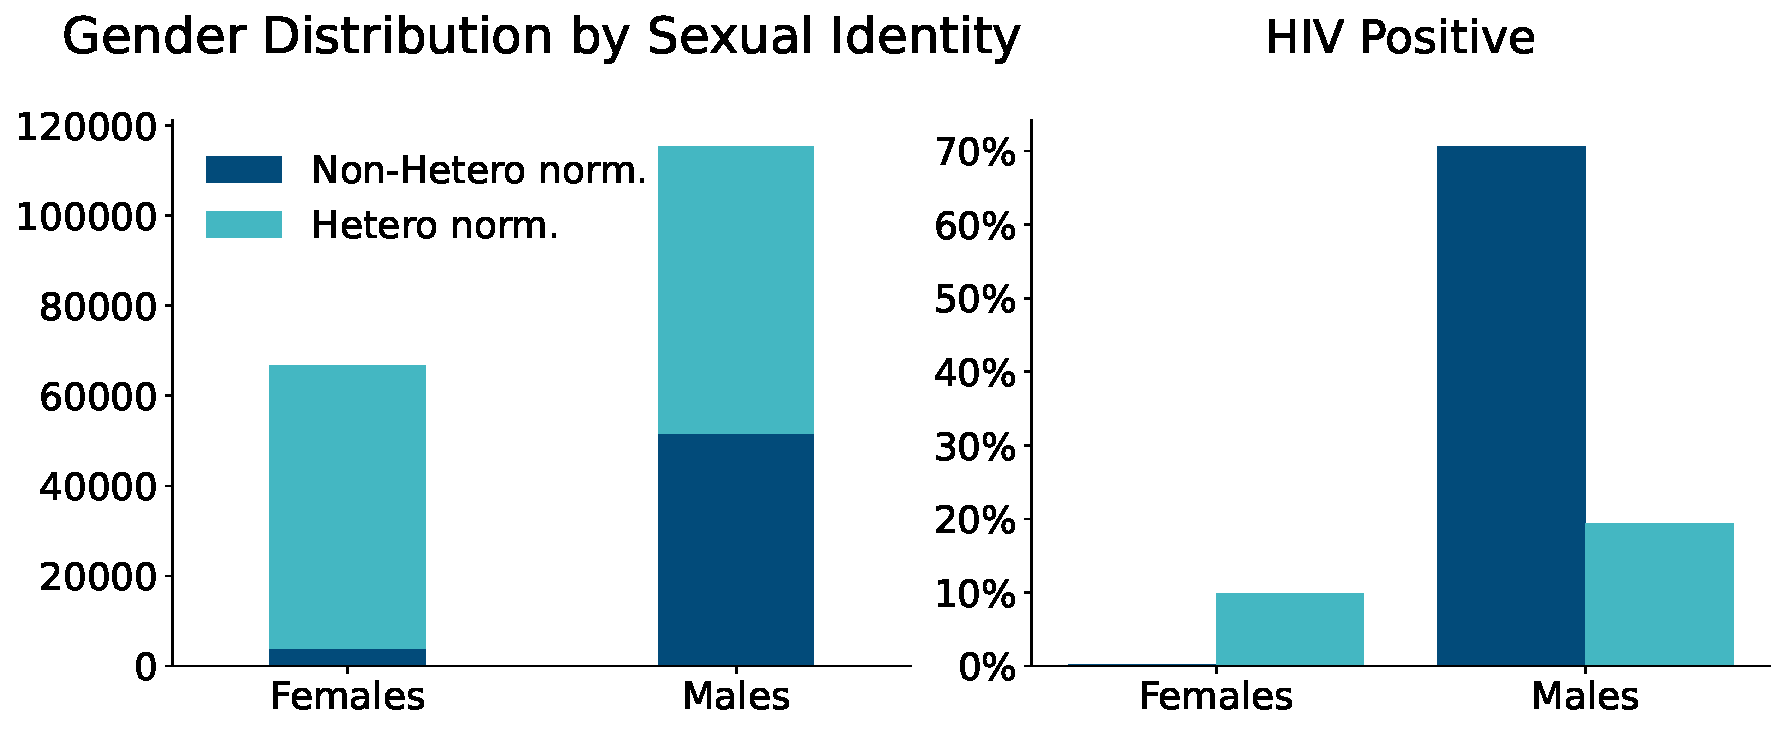
\includegraphics{HIVPaper_files/figure-latex/fig-demography-output-1.pdf}

}

\caption{\label{fig-demography}The left plot shows the dataset's gender
and sexual identity distribution, while the right plot displays the
ratio among those who tested positive.}

\end{figure}

\hypertarget{exploring-hiv-risk-factors-and-predictors}{%
\section{Exploring HIV Risk Factors and
Predictors}\label{exploring-hiv-risk-factors-and-predictors}}

Let's begin by constructing a model aimed at predicting HIV infection
based on known variables: gender and sexual identity. All statistical
models in this project were built using the \texttt{numpyro} package in
Python.\footnote{It's a simplified version of the \texttt{pyro} package,
  both of which focus on providing tools for probabilistic data
  analysis, including the creation of advanced hierarchical models. The
  package documentation can be found
  \href{https://num.pyro.ai/en/latest/index.html\#introductory-tutorials}{here}.}
The Bayesian logistic regression model below examines the interplay
between HIV infection (HIV), heteronormativity (Hetero\_normative), and
gender (Gender\_encoded). All of my models follow the same template.
Model parameters include the intercept term \texttt{a} representing
baseline log-odds of HIV infection, coefficients \texttt{b} and
\texttt{c} quantifying the effects of heteronormativity and gender,
respectively. The logit transformation combines these factors to
calculate log-odds. Priors in the form of normal distributions are
assigned to model parameters. When it comes to priors, I have selected
modest parameters that have a limited impact on the posterior
distributions. The relatively large size of the dataset exerts a more
substantial influence. A binomial likelihood function is used for
observed HIV infection data, updating parameter beliefs. The model is
run using the No-U-Turn Sampler (NUTS), a variant of Markov Chain Monte
Carlo (MCMC). Here's a template of what the model looks like:

\footnotesize

\begin{Shaded}
\begin{Highlighting}[]
\NormalTok{dat\_listGender }\OperatorTok{=}\NormalTok{ \{}
    \StringTok{\textquotesingle{}HIV\textquotesingle{}}\NormalTok{: PKD\_model\_DF.HIV.values,}
    \StringTok{\textquotesingle{}Hetero\_normative\textquotesingle{}}\NormalTok{: PKD\_model\_DF.Hetero\_normative.values,}
    \StringTok{\textquotesingle{}Gender\_encoded\textquotesingle{}}\NormalTok{: PKD\_model\_DF.Gender\_encoded.values,}
\NormalTok{    \}}

\KeywordTok{def}\NormalTok{ model\_hetero\_Gender(Hetero\_normative, Gender\_encoded, HIV}\OperatorTok{=}\VariableTok{None}\NormalTok{):     }
\NormalTok{    a }\OperatorTok{=}\NormalTok{ numpyro.sample(}\StringTok{"a"}\NormalTok{, dist.Normal(}\DecValTok{0}\NormalTok{, }\FloatTok{1.5}\NormalTok{))  }
\NormalTok{    b }\OperatorTok{=}\NormalTok{ numpyro.sample(}\StringTok{"b"}\NormalTok{, dist.Normal(}\DecValTok{0}\NormalTok{, }\FloatTok{0.5}\NormalTok{).expand([}\DecValTok{2}\NormalTok{])) }
\NormalTok{    c }\OperatorTok{=}\NormalTok{ numpyro.sample(}\StringTok{"c"}\NormalTok{, dist.Normal(}\DecValTok{0}\NormalTok{, }\FloatTok{0.5}\NormalTok{).expand([}\DecValTok{2}\NormalTok{])) }

\NormalTok{    logit\_p }\OperatorTok{=}\NormalTok{ a }\OperatorTok{+}\NormalTok{ b[Hetero\_normative] }\OperatorTok{+}\NormalTok{ c[Gender\_encoded]}
\NormalTok{    numpyro.sample(}\StringTok{"HIV"}\NormalTok{, dist.Binomial(logits}\OperatorTok{=}\NormalTok{logit\_p), obs}\OperatorTok{=}\NormalTok{HIV)}

\NormalTok{HIV\_HetreoNorm\_Gender }\OperatorTok{=}\NormalTok{ MCMC(NUTS(model\_hetero\_Gender),}
\NormalTok{    num\_warmup}\OperatorTok{=}\DecValTok{500}\NormalTok{, num\_samples}\OperatorTok{=}\DecValTok{500}\NormalTok{) }
\NormalTok{HIV\_HetreoNorm\_Gender.run(random.PRNGKey(}\DecValTok{0}\NormalTok{), }\OperatorTok{**}\NormalTok{dat\_listGender)}
\end{Highlighting}
\end{Shaded}

\normalsize

Now, let's explore the relationship between our demographic predictors
and the likelihood of being HIV positive. In
Figure~\ref{fig-modelsexhetero}, you can examine the predictions
generated by the model, which incorporated gender and sexual identity as
predictors. The violin plots depict the distribution of predictions,
reflecting the marginal posterior densities derived through sampling
techniques, rather than providing single point estimates. This approach
aligns with the Bayesian methodology, as it conveys more information
than, for instance, just a mean or statistical tests.

\begin{figure}[H]

{\centering 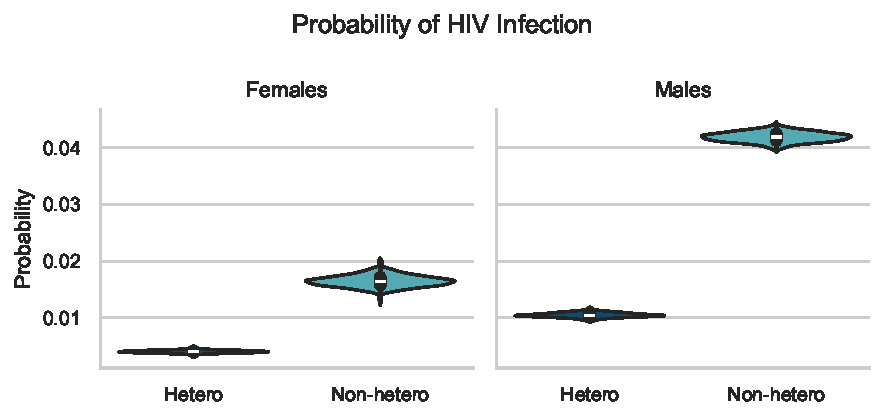
\includegraphics{HIVPaper_files/figure-latex/fig-modelsexhetero-output-1.pdf}

}

\caption{\label{fig-modelsexhetero}This visualization displays the
predictions generated by the logistic regression model trained on the
dataset. The violins depict the probability distribution of HIV
acquisition predictions with respect to gender and sexual identity.}

\end{figure}

Comparatively, the differences are easily visible, with non-heterosexual
males appearing to be at the highest risk of infection when we consider
no other factors. However, there are also distinctions between genders,
with males once again being at greater risk. In fact, there are many
publications supporting the claim that women are less susceptible to
infection compared to men (Beyrer et al. 2012). The risk of a woman
contracting HIV during intercourse with an infected person is lower than
that for a man.

\begin{figure}

{\centering 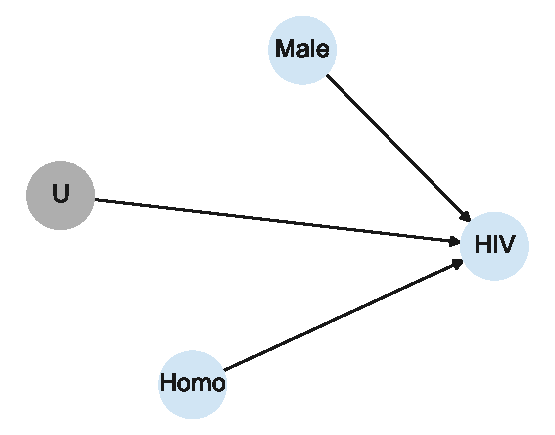
\includegraphics{HIVPaper_files/figure-latex/fig-dagwrong-output-1.pdf}

}

\caption{\label{fig-dagwrong}DAG representing the naive relation between
variables resembling the first model. `U' stands for unobserved,
\textasciitilde H for non-hetero, while the rest of the labels are
self-explanatory.}

\end{figure}

But does this information provide us with insights into causal
relationships? It certainly provides some insights, but we should
consider a wide range of underlying causes that might be responsible for
such results. Let's examine a Directed Acyclic Graph (DAG), represented
as Figure~\ref{fig-dagwrong}, which corresponds to the rationale of the
initial model.

The reasoning appears to be somewhat limited, suggesting that there is
something `special' about males and non-heterosexual individuals that
makes them more prone to HIV infection. The node representing
`Unobserved' deserves special attention, as it encompasses all other
potential factors that could lead to an HIV infection, such as
transmission through a used needle. The primary achievement of this
reasoning is to reinforce the stereotype that HIV is primarily an
infection of homosexual males. Let's now shift our focus to the main
objective of this work. We aim to identify predictors that may offer a
better explanation for HIV infection, potentially going beyond the
simplistic division between heterosexual and non-heterosexual
individuals.

What predictors should we consider? The risk factors for HIV have been
the subject of numerous studies, and we can leverage their findings in
our analysis. According to the World Health Organization (WHO), the most
common risk factors include:

\begin{quote}
\begin{itemize}
\tightlist
\item
  having condomless anal or vaginal sex;
\item
  having another sexually transmitted infection (STI) such as syphilis,
  herpes, chlamydia, gonorrhoea and bacterial vaginosis;
\item
  engaging in harmful use of alcohol and drugs in the context of sexual
  behaviour;
\item
  sharing contaminated needles, syringes and other injecting equipment
  and drug solutions when injecting drugs;
\item
  receiving unsafe injections, blood transfusions and tissue
  transplantation, and medical procedures that involve unsterile cutting
  or piercing; and
\item
  experiencing accidental needle stick injuries, including among health
  workers. ({``{H}{I}{V} and {A}{I}{D}{S} --- Who.int''} 2023)
\end{itemize}
\end{quote}

Since we are specifically interested in examining transmission based on
sexual activities, we will exclude injective drug users and marginal
cases of medical accidents where infection might occur through contact
with a patient's blood. However, we can add the variable representing
the number of sexual partners (per year) a person has. The rationale
here is simple: more partners mean more opportunities for infection.
Additionally, we will focus on anal sex as a chosen risk factor, given
that it is the most high-risk sexual activity.\footnote{We could have
  considered oral sex and the risk of not using protection during oral
  sex, but due to the ambiguous distinction between passive and active
  oral sex, the data variable seems unreliable. There is common
  confusion between what constitutes passive and active oral sex. By
  definition, being on the receptive end is called passive, while using
  one's mouth is called active. However, in the gay community, the
  division between tops and bottoms (actives and passives) often
  perceives receptive oral sex as an active activity.}

\begin{figure}

{\centering 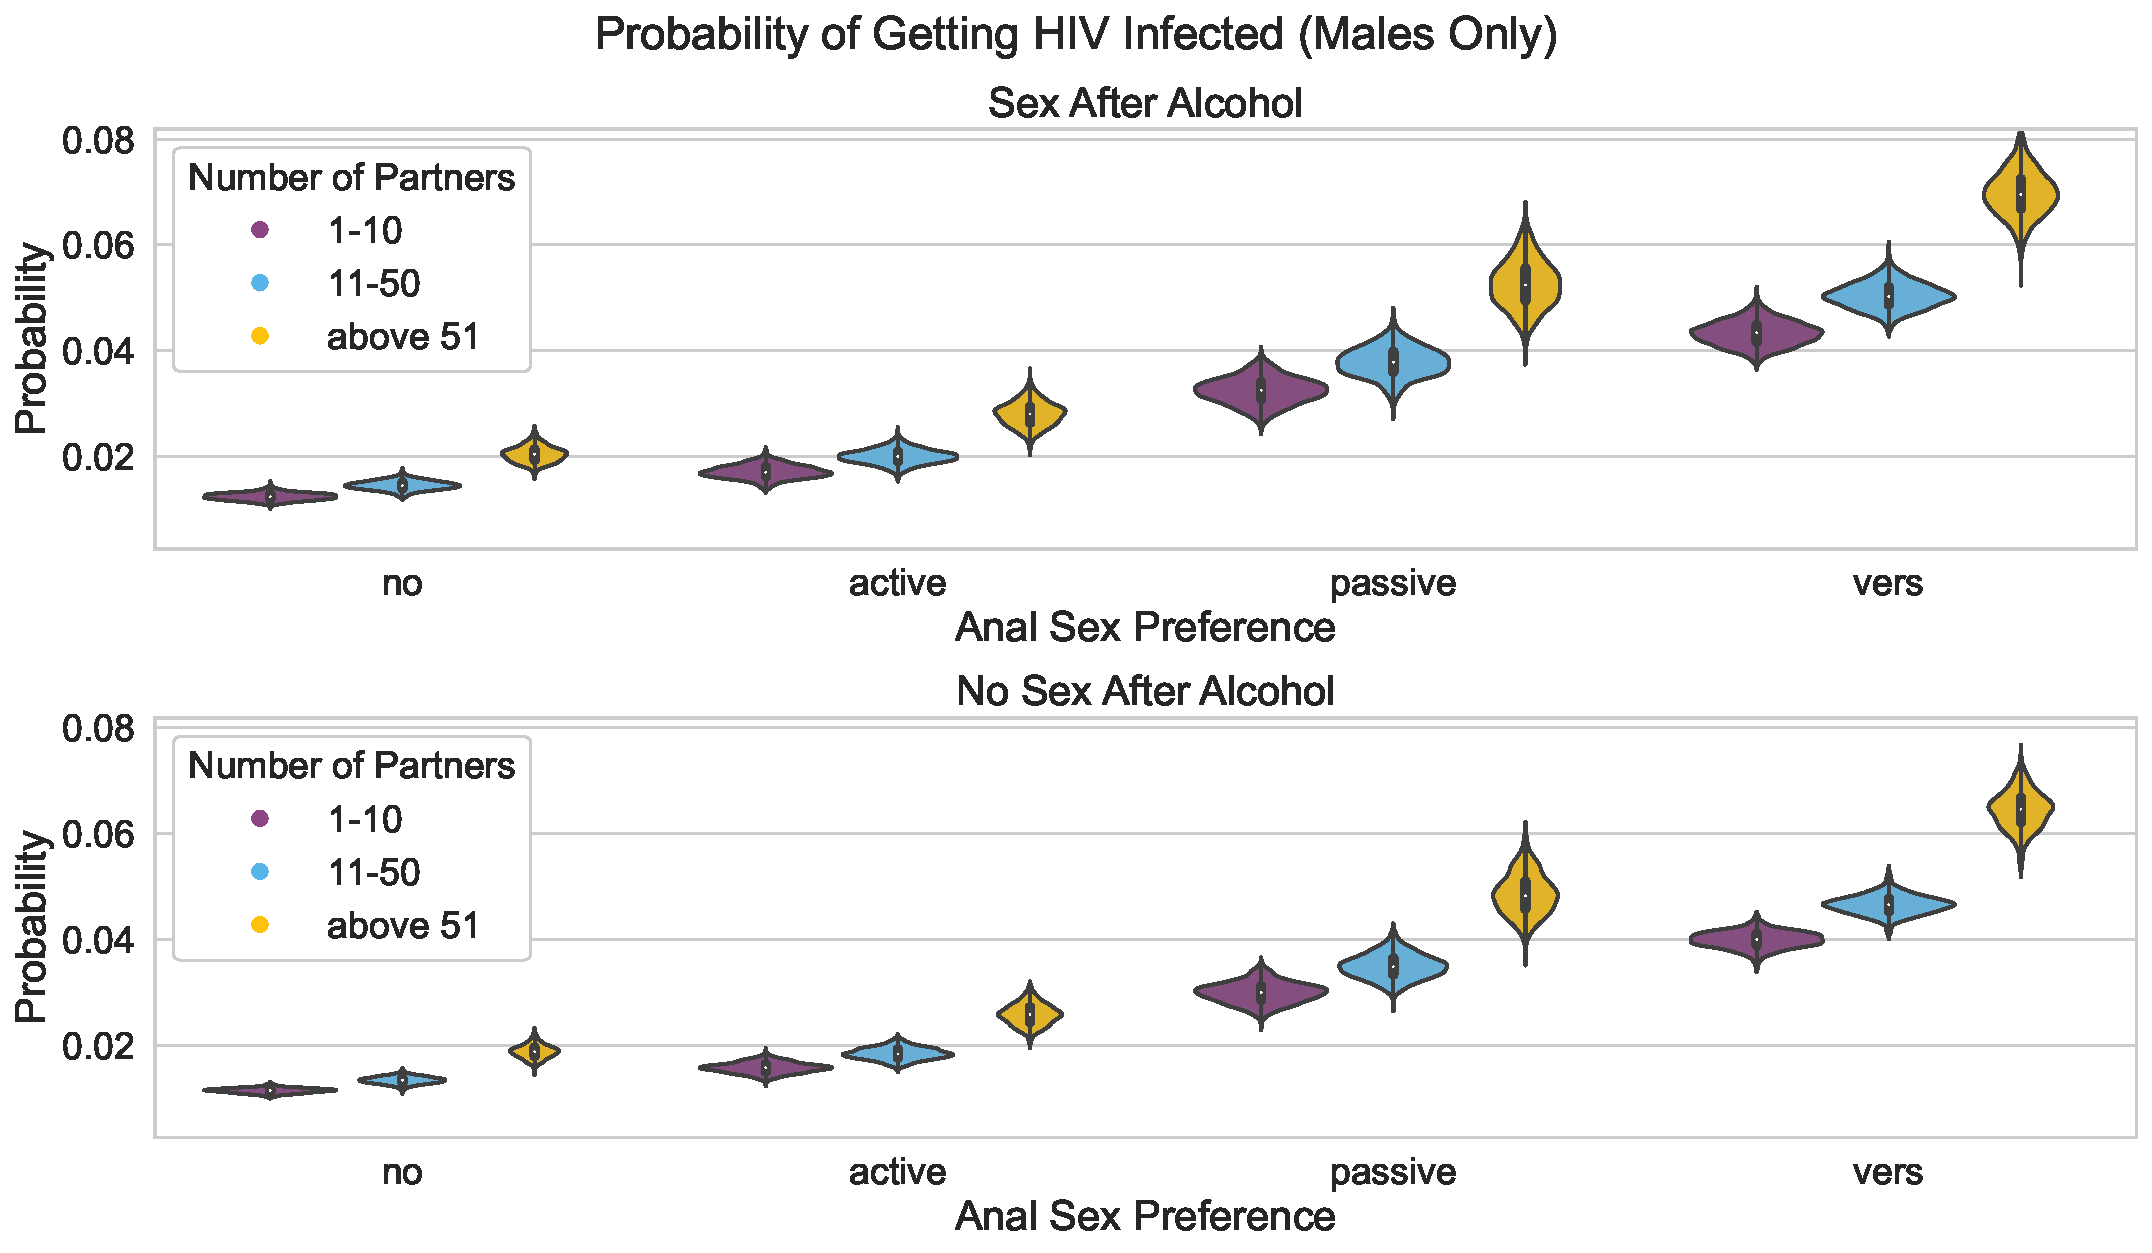
\includegraphics{HIVPaper_files/figure-latex/fig-violinbigmales-output-1.pdf}

}

\caption{\label{fig-violinbigmales}In this visualization, you can
observe various categories considered as contributors to a risky
profile. This plot focuses solely on males.}

\end{figure}

\begin{figure}

{\centering 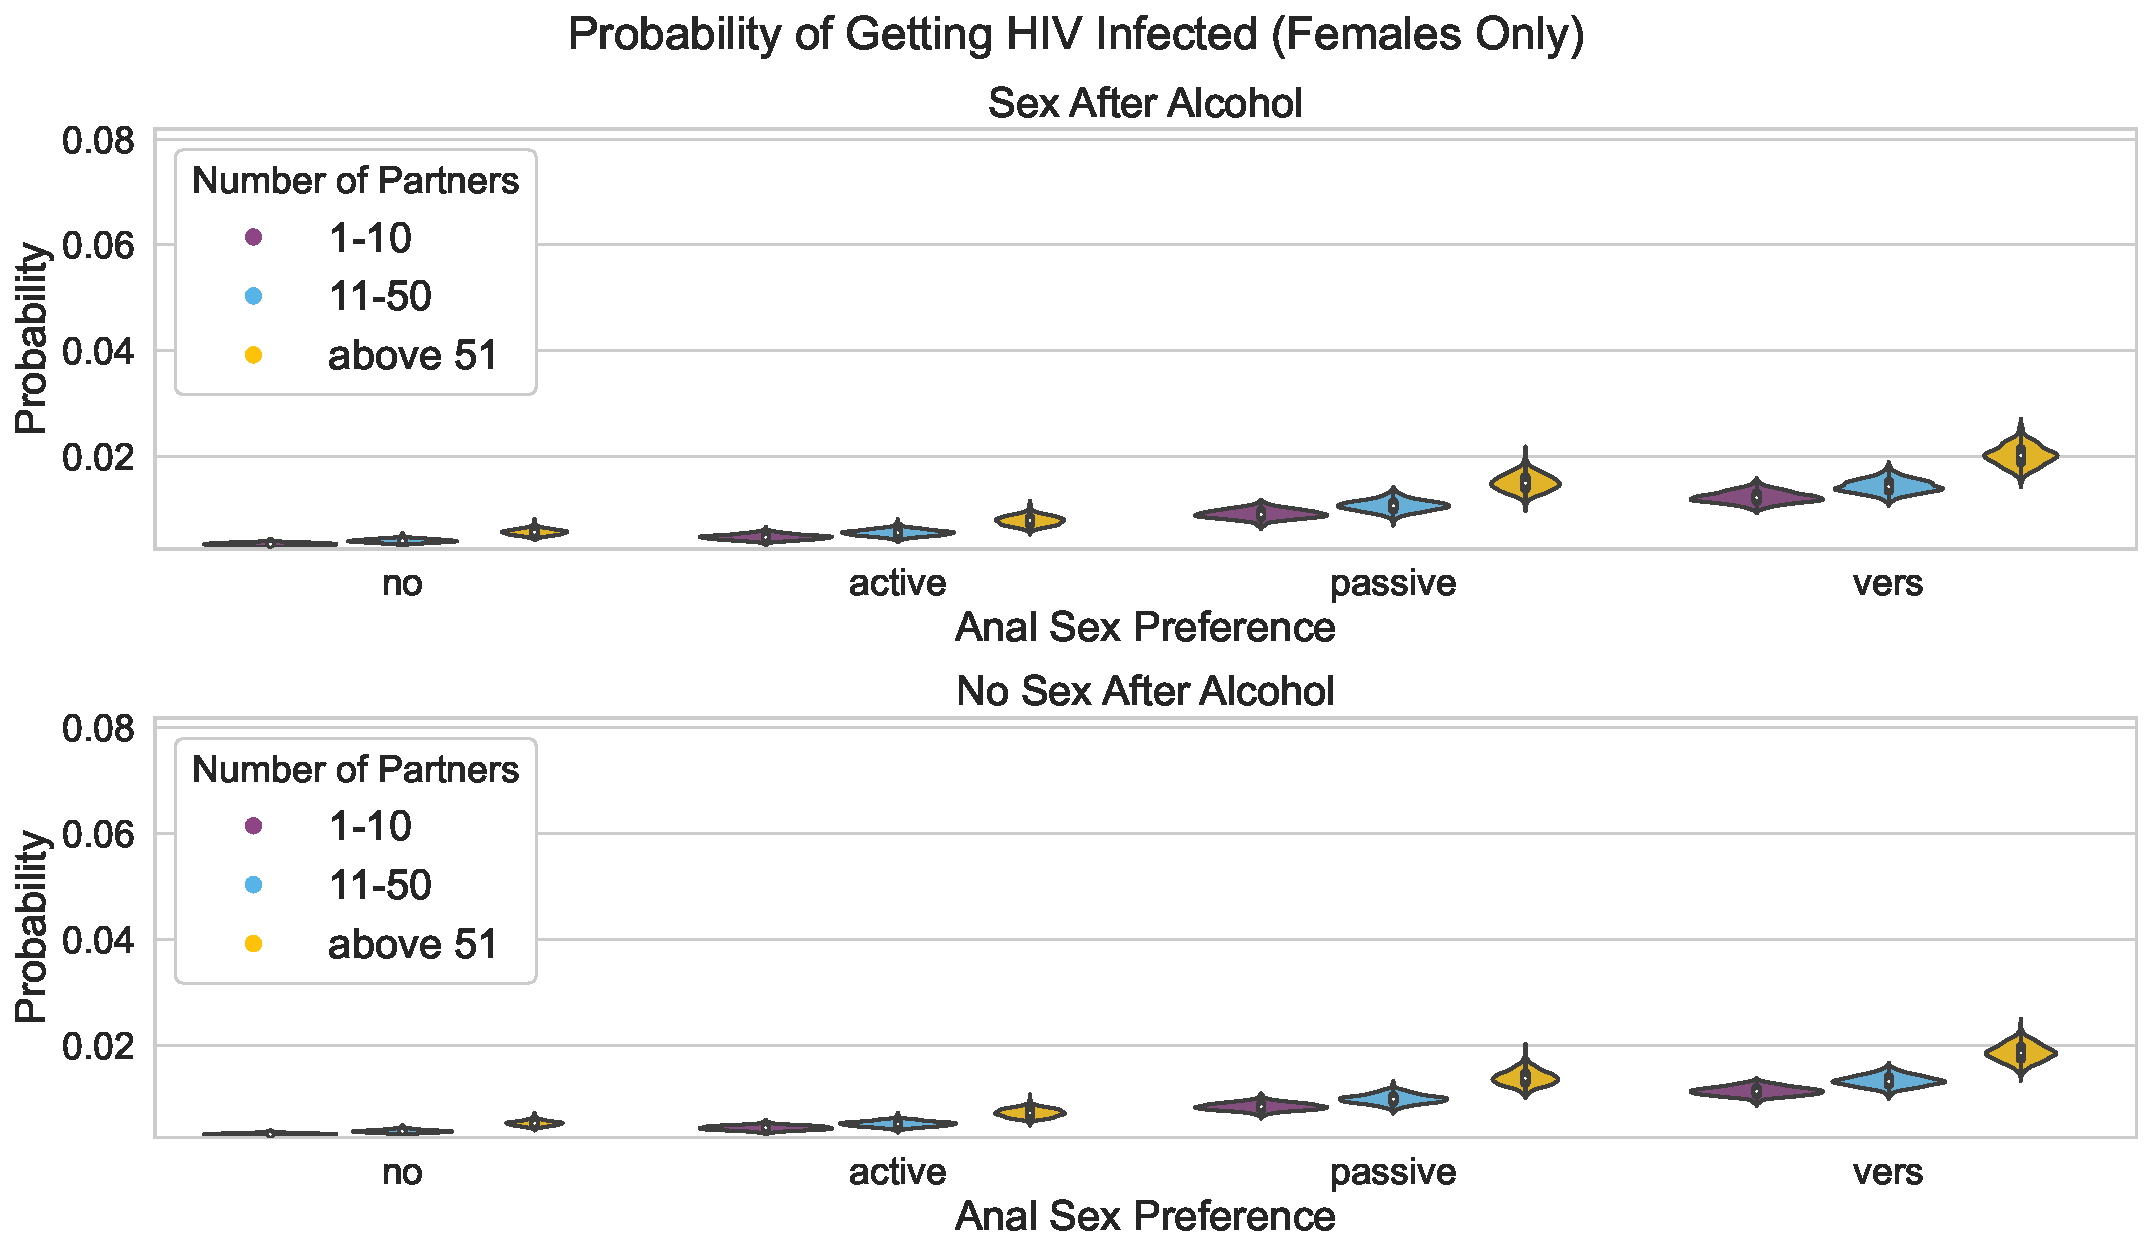
\includegraphics{HIVPaper_files/figure-latex/fig-violinbigfemales-output-1.pdf}

}

\caption{\label{fig-violinbigfemales}This is a twin visualization
covering risky categories. This plot focuses exclusively on females, and
the difference in the probability of getting infected is striking.}

\end{figure}

In figures: Figure~\ref{fig-violinbigmales} and
Figure~\ref{fig-violinbigfemales}, you can observe visualizations of
predictions created by the logistic regression model for males and
females, respectively. The model utilized the following predictors:
gender, binned number of sexual partners (per year), preference for anal
intercourse, and engaging in sexual activity under the influence of
alcohol. There is a striking contrast between males and females. Even
when women fall into the most high-risk profile category, the risk of
infection remains considerably lower than for males. As mentioned
earlier, studies support these findings, suggesting that women are
significantly less susceptible to HIV infection for biochemical reasons.

All these factors contribute to the definition of the most high-risk
profile: a male with more than 51 sexual partners, a preference for
versatile anal intercourse, and engaging in alcohol-induced sex. It's
evident that each of these categories individually increases the
probability of infection.

\hypertarget{defining-a-high-risk-profile-for-hiv-infection}{%
\section{Defining a High-Risk Profile for HIV
Infection}\label{defining-a-high-risk-profile-for-hiv-infection}}

The next step involves defining a Risk Profile (RP) that maximizes the
chances of HIV infection. This profile will
\textbf{ exclude sexual identity and gender} in order to empasize the
influence of other variables. I will introduce the profile as a new
binary variable in the dataset. This approach is simpler than
constructing a model that accommodates all these variables and creates
different categories for each of them.

The variables I will use to create the RP are:

\begin{itemize}
\tightlist
\item
  Alcochol-induced sex,
\item
  Having more than 10 sexual partners per year,
\item
  Anal sex preference: passive or versatile,
\item
  Anal sex protection use: sometimes or never.
\end{itemize}

\begin{figure}

{\centering 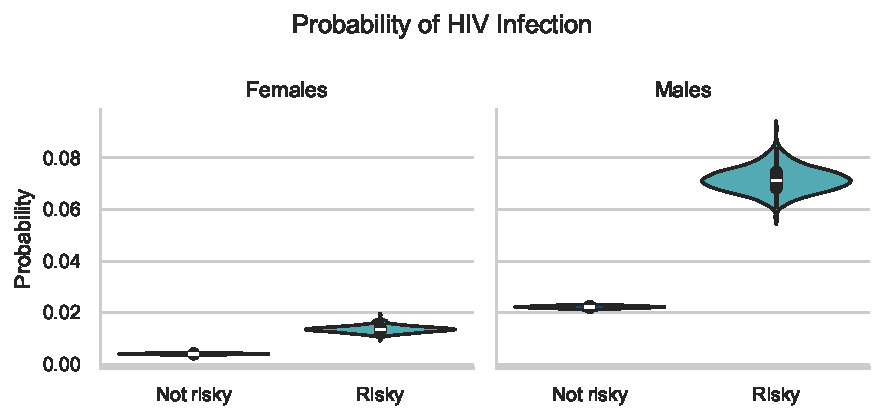
\includegraphics{HIVPaper_files/figure-latex/fig-riskprofgenderhiv-output-1.pdf}

}

\caption{\label{fig-riskprofgenderhiv}The visualization represents the
probability of getting infected for RP holders, divided into females and
males.}

\end{figure}

In Figure~\ref{fig-riskprofgenderhiv}, which represents the probability
of infection for the RP, we can observe that the probability for males
in the RP group is higher than the probability in our first model
(represented in Figure~\ref{fig-modelsexhetero}), which showed a high
probability of infection for non-hetero males. This suggests that RP
profile holders are at a greater risk of infection than non-hetero
males. But what is the relationship between these two variables? We will
test this with our next model.

\begin{figure}

{\centering 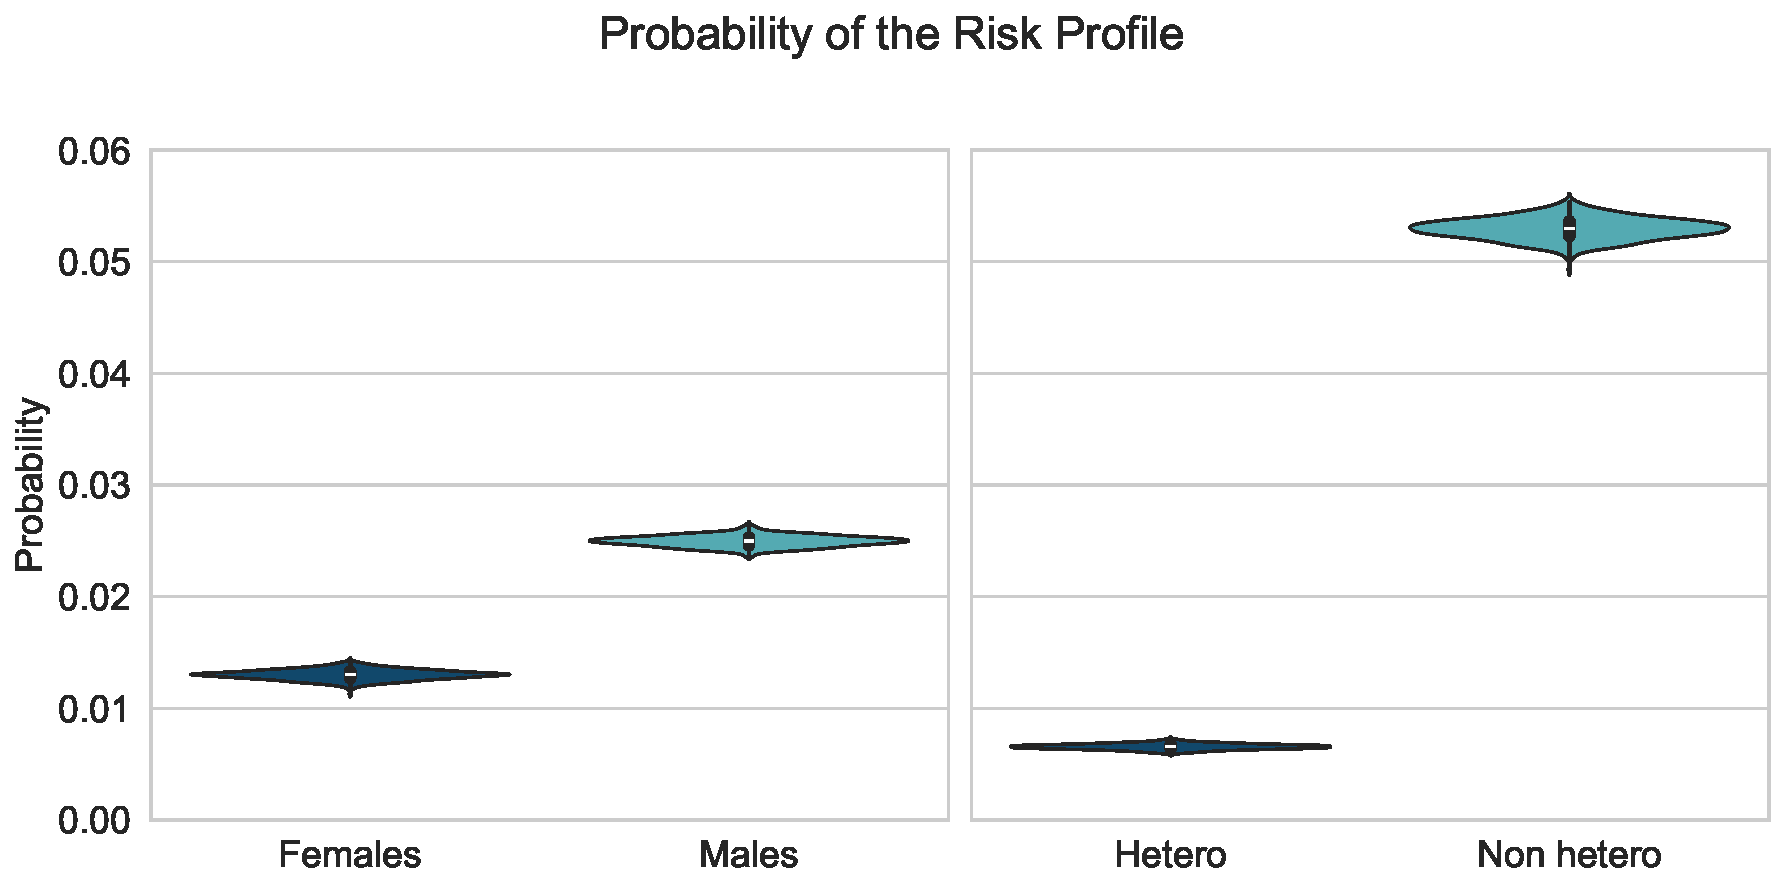
\includegraphics{HIVPaper_files/figure-latex/fig-twinriskprob-output-1.pdf}

}

\caption{\label{fig-twinriskprob}The visualization represents the
probability of being in RP, with a division by gender on the left and by
sexual identity on the right.}

\end{figure}

In the pair of visualizations in Figure~\ref{fig-twinriskprob}, we can
see the models that were given gender and sexual identity as predictors
to predict being in the most risky group. As it can be seen, non-hetero
individuals and males have the highest probability of being in that
group.

Returning to representing the causes of HIV infection, the variables
that increase the probability of infection are better at getting you
infected. Therefore, considering them as causes is more reasonable. The
Directed Acyclic Graph (DAG) that will represent the relationship
between the considered variables, after our analysis, will look
something like the one shown in Figure~\ref{fig-postdag}.

\begin{figure}

{\centering 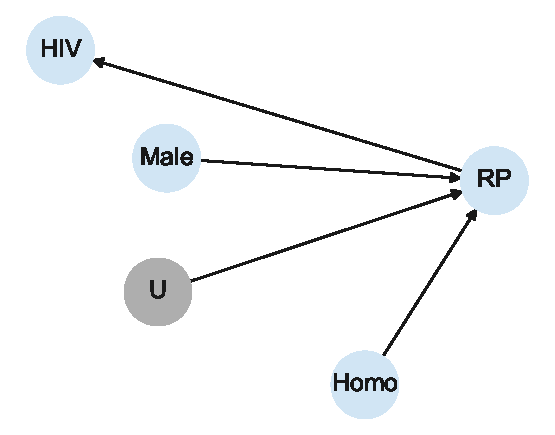
\includegraphics{HIVPaper_files/figure-latex/fig-postdag-output-1.pdf}

}

\caption{\label{fig-postdag}This DAG represents the relationship between
demographic variables, the RP (risk profile), and HIV infection.}

\end{figure}

\hypertarget{conclusions}{%
\section{Conclusions}\label{conclusions}}

In the Figure~\ref{fig-postdag}, the DAG represents the relationship
between the predictors we analyzed. It seems to represent cause and
effect more realistically than just relying on the notion that
non-hetero males are `special' in some way, leading to HIV infection. In
fact, non-hetero males have a high probability of being in an RP group,
and risky behaviors associated with RP status are the causes of HIV
infection. This includes having anal intercourse and a high number of
sexual partners, which is associated with non-hetero males. The reason
why non-hetero males choose to be in that group is not known,
represented by the Unobserved node.

Is the stereotype true then? Well, non-hetero males are at the highest
risk of getting HIV infected, but their sexual identity is not a direct
cause of that. Hetero sexual males who enjoy similar activities, and
thus are in an RP, also have higher chances of getting infected. The
more direct cause is risky behavior, and non-hetero males tend to engage
in more risky behaviors. Therefore, the story is more complex. The
findings of this paper support the claim that:
\textbf{the sole fact of being a non-hetero person does not make you more susceptible to getting HIV infected}.

An interesting observation in the field of interest to specialists from
different scientific branches is the fact that women get infected far
less often than males.

One thing worth noting is the concerning growth of new HIV infections in
Europe. The mentioned stereotype might have a negative effect on public
opinion, as hetero people might feel too confident about not getting
infected, assuming this infection is mainly associated with non-hetero
males. This analysis has shown that there is a risky behavior pattern
that all people should be aware of, as it can lead to HIV infection. In
fact, as we have seen at the beginning, hetero males tend to test
themselves much less often than non-hetero males.

\hypertarget{appendix}{%
\section{Appendix}\label{appendix}}

In this appendix, I present additional visualizations that provide
further insights into the dataset used in our analysis, aligning with
the principles of Exploratory Data Analysis (EDA).

The first visualization, presented in Figure~\ref{fig-agehist} , depicts
the age distribution among all PKD clients. It is apparent that a
substantial number of clients undergoing testing fall within the age
brackets of their 20s and 30s. The 95\% confidence interval for age
spans from 19 to 55 years.

\begin{figure}

{\centering 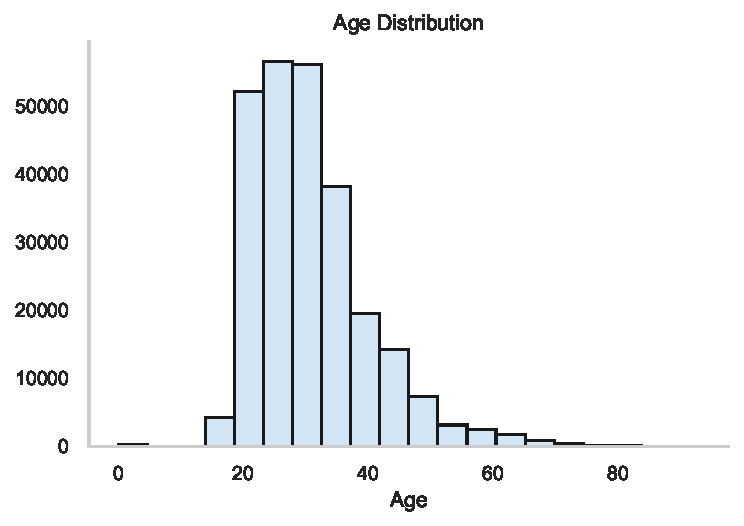
\includegraphics{HIVPaper_files/figure-latex/fig-agehist-output-1.pdf}

}

\caption{\label{fig-agehist}Histogram of age distribution among PKD
clients, the 95\% confidence interval is between 19 and 55 years of
age.}

\end{figure}

Figure~\ref{fig-causes} delves into the motivations driving clients to
seek HIV testing at PKD facilities. It's worth noting that many clients
cite multiple reasons, e.g.~both heterosexual and homosexual intercourse
as the cause of their visit. To present a clear picture, these causes
have been aggregated to highlight the most prevalent motivations for
testing.

Figure~\ref{fig-causes} also provides percentages indicating the portion
of clients with a specific motivation who received a positive test
result. Notably, clients whose partners tested positive exhibit the
highest percentage of positive results. it's worth mentioning that there
were 0 cases of positive results among sex worker-related testing. This
could be attributed to both a low number of clients motivated by this
cause (less than 100) and a cautious approach to sexual health,
potentially involving the use of PrEP.

\begin{figure}

{\centering 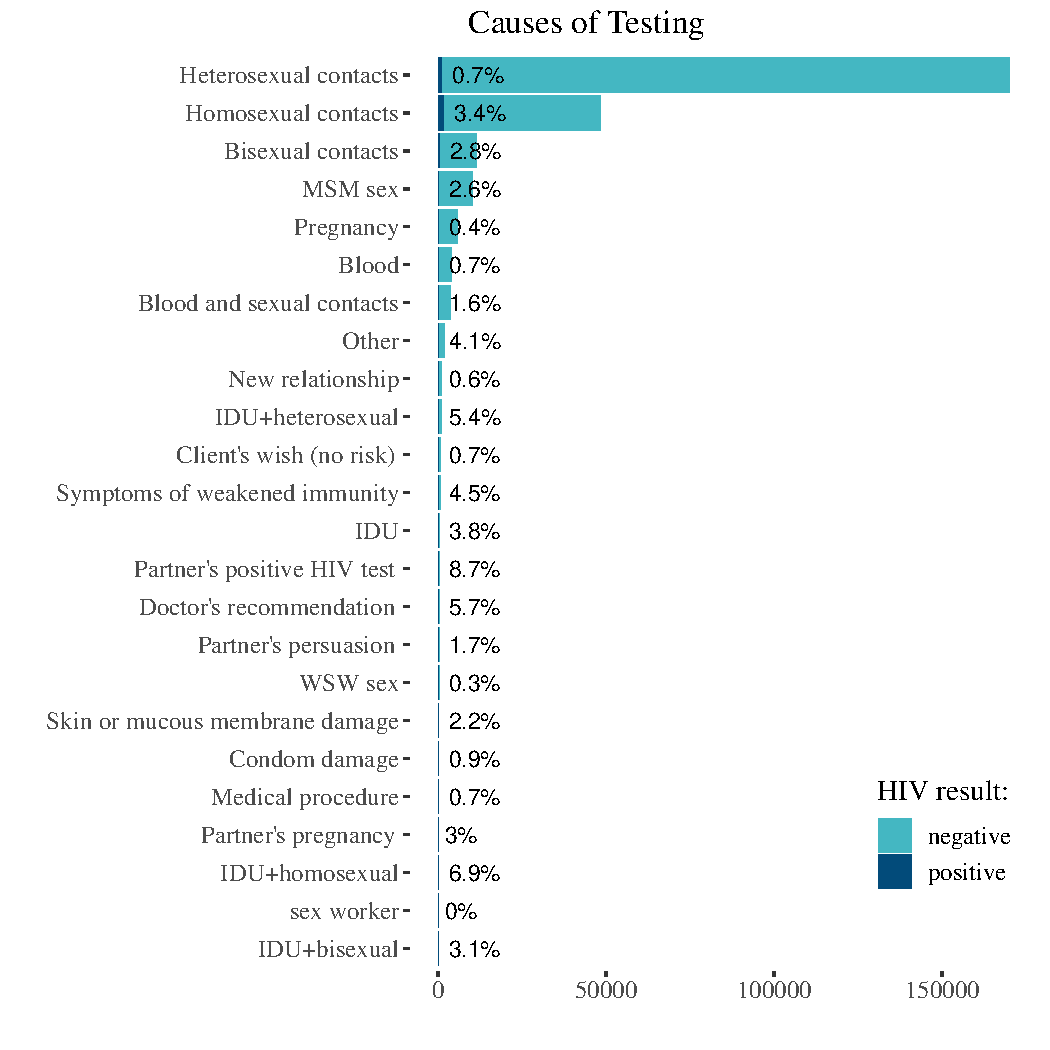
\includegraphics[width=0.85\textwidth,height=\textheight]{../visualizations/causesplott.pdf}

}

\caption{\label{fig-causes}Causes that motivated clients to test for HIV
at PKD test centers (IDU stands for Injective Drug User).}

\end{figure}

\pagebreak

\hypertarget{references}{%
\section*{References}\label{references}}
\addcontentsline{toc}{section}{References}

\hypertarget{refs}{}
\begin{CSLReferences}{1}{0}
\leavevmode\vadjust pre{\hypertarget{ref-Beyrer2012}{}}%
Beyrer, Chris, Stefan D Baral, Frits van Griensven, Steven M Goodreau,
Suwat Chariyalertsak, Andrea L Wirtz, and Ron Brookmeyer. 2012.
{``Global Epidemiology of {HIV} Infection in Men Who Have Sex with
Men.''} \emph{The Lancet} 380 (9839): 367--77.
\url{https://doi.org/10.1016/s0140-6736(12)60821-6}.

\leavevmode\vadjust pre{\hypertarget{ref-EUHIV20212022}{}}%
European Centre for Disease Prevention and Control, and World Health
Organization. 2022. \emph{HIV/AIDS Surveillance in Europe 2022\,: 2021
Data}. European Centre for Disease Prevention; Control.
\url{https://doi.org/10.2900/818446}.

\leavevmode\vadjust pre{\hypertarget{ref-unaidsGlobalAIDS}{}}%
{``{G}lobal {H}{I}{V} \& {A}{I}{D}{S} Statistics --- {F}act Sheet ---
Unaids.org.''} 2023.
\url{https://www.unaids.org/en/resources/fact-sheet}.

\leavevmode\vadjust pre{\hypertarget{ref-whoAIDS}{}}%
{``{H}{I}{V} and {A}{I}{D}{S} --- Who.int.''} 2023.
\url{https://www.who.int/news-room/fact-sheets/detail/hiv-aids}.

\leavevmode\vadjust pre{\hypertarget{ref-Sharp2011}{}}%
Sharp, P. M., and B. H. Hahn. 2011. {``Origins of {HIV} and the {AIDS}
Pandemic.''} \emph{Cold Spring Harbor Perspectives in Medicine} 1 (1):
a006841--41. \url{https://doi.org/10.1101/cshperspect.a006841}.

\end{CSLReferences}



\end{document}
